
\section{Practicality Evaluation: Case Studies}
\label{sec-case}

This section evaluates \app's practicality through
%performing independence auditing to redundancy deployments in
three small but realistic case studies with respect to
unexpected common
network, hardware, and software dependencies, respectively.

\begin{figure}[tb] \centering
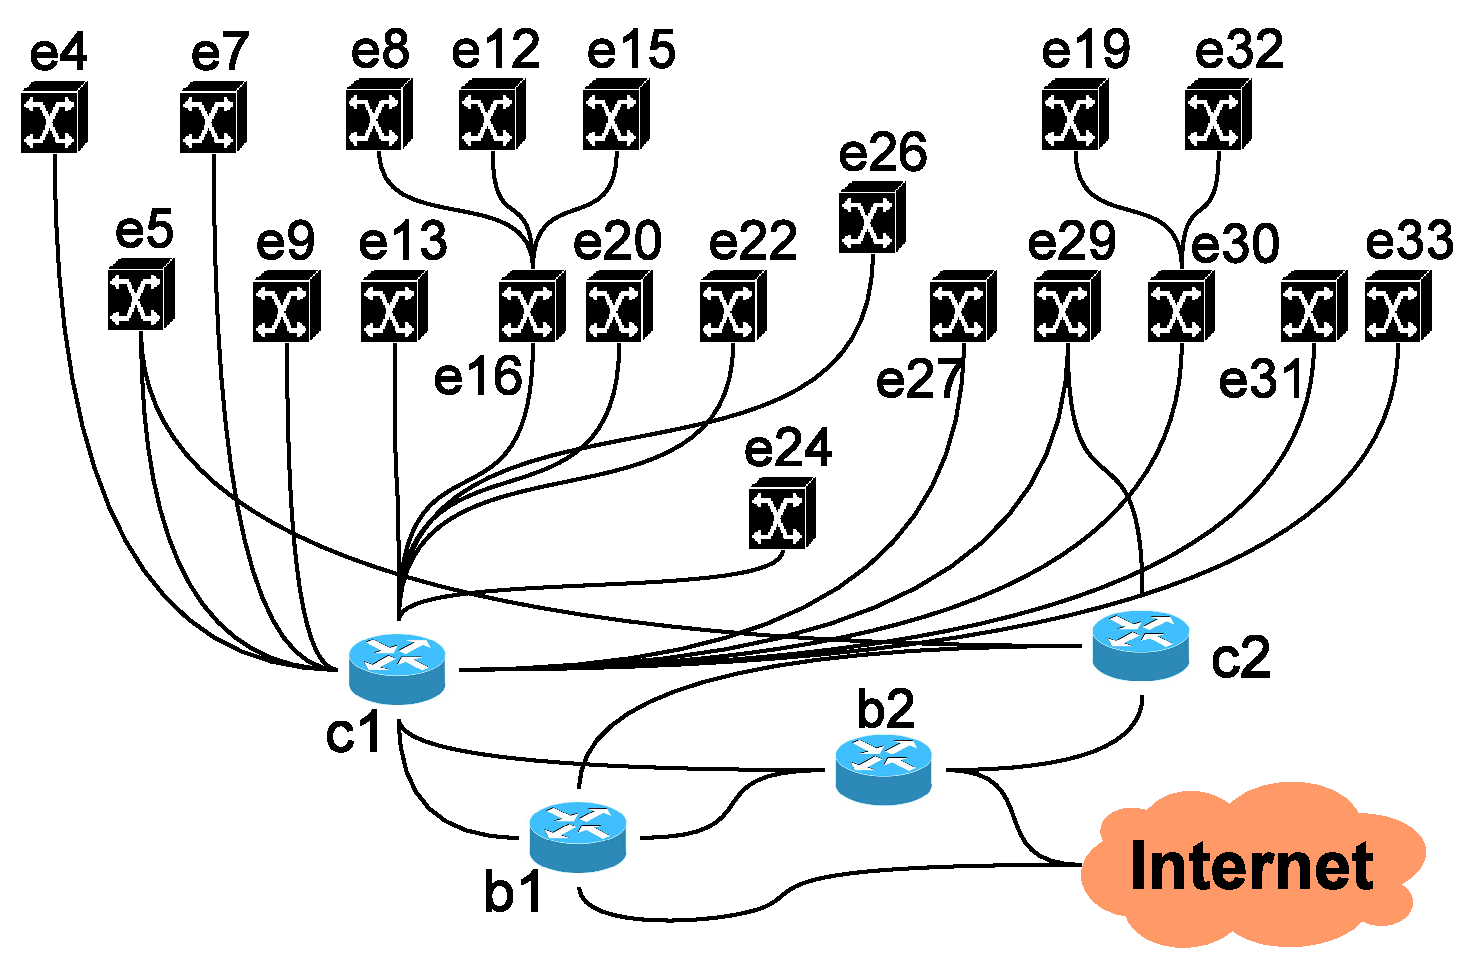
\includegraphics[width=0.94\textwidth]{figs/enterprise.eps}
\caption{Case study for common network dependency.}
\label{fig-case1}
\end{figure}

\subsection{Common Network Dependency}
\label{subsec-case1}

Our first case study targets a scenario
similar to the example given in the introduction.
A data center operator, Alice, wants to deploy a new service $S$
in her data center, and replicates the critical states of $S$ across
two servers within her data center.
Before service deployment,
Alice uses \app to structurally audit
the data center network in order to avoid
potential correlated failures resulting from common
network dependencies.
%~(switches in this case).
We used a real data center topology~\cite{benson10network} to model
Alice's data center network.
As shown in Figure~\ref{fig-case1},
this data center has many Top-of-Rack (ToR) switches (\ie, e1-e33)
each of which is connected to an individual rack.
There are four core routers (\ie, b1, b2, c1, and c2)
connecting ToR switches to the Internet.
%Suppose
%intends to build a two-way replication for her service.
%In order to avoid correlated failure risks,
%she consults \app by submitting a specification.

The \app first collects network dependencies, and then
executes the \sia protocol to provide auditing at the \ft level.
The auditing report generated by our prototype, based on the
failure sampling algorithm (which we ran for $10^6$ rounds)
and the size-based ranking algorithm,
suggests that
\{Rack~5, Rack~29\} is the most-independent deployment in this scenario.
Without \app, it is highly possible that Alice
builds a two-way replication with unexpected \rgs.
For instance, if she uses redundancy \{Rack~4, Rack~7\},
the failure of C1 would invalidate her efforts.

A formal analysis indicates that
there are 190 different two-way redundancy deployments, among which 27
do not have unexpected \rgs.
This means, without \app, a random selection leads to only 14\% probability
for Alice to avoid correlated failures.
Furthermore, if we assume the failure probability of all
network devices is 0.1, the redundancy deployment
\{Rack~5, Rack~29\} is indeed the one
with the lowest failure probability.


\subsection{Common Hardware Dependency}
\label{subsec-case2}

\begin{figure}[tb] \centering
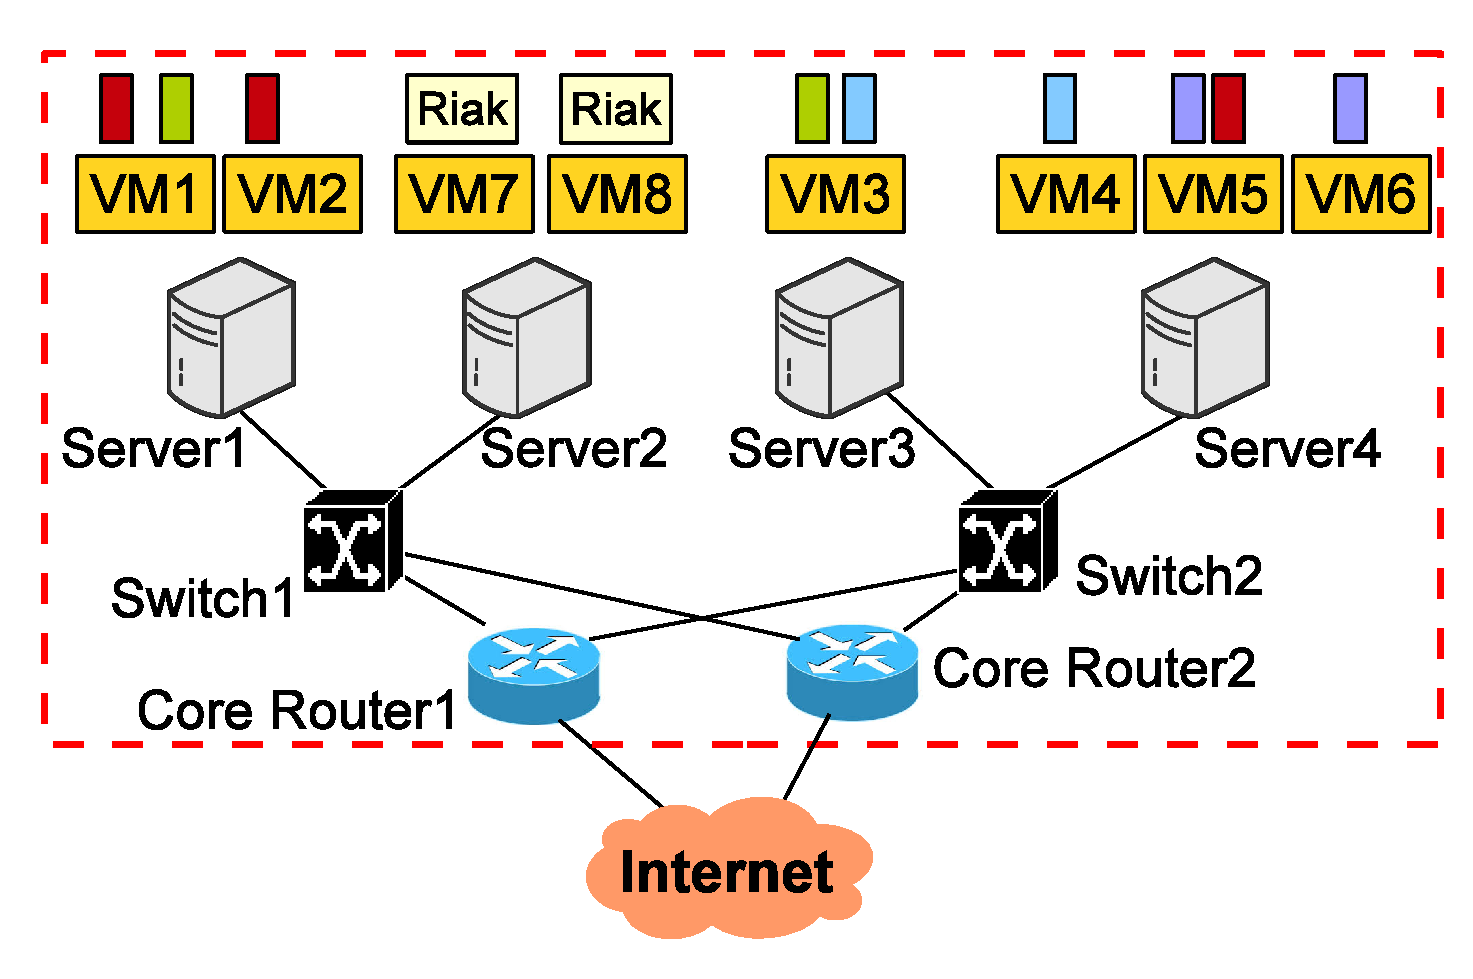
\includegraphics[width=0.94\textwidth]{figs/campus.eps}
\caption{Case study for common hardware dependency.}
\label{fig-case2}
\end{figure}

As shown in Figure~\ref{fig-case2},
we have built a simple IaaS cloud in the lab with four servers
and four switches.
While perhaps not an impressive cloud,
this configuration as will be shown
sufficiently exercises the \app prototype.
We used OpenStack to support the automatic virtual machine (VM) management,
and deployed various services on VMs for different uses.
OpenStack automatically handles the allocation of resources,
and thus Alice simply provides virtual machine images
containing the services to the cloud.
In particular, we deployed an S3-like Riak~\cite{Riak}
cloud storage service.
%which provides storage service similar to S3.
%The service is built on a well-known storage
%system called Riak~\cite{Riak}.
For redundancy, Riak was run on two VMs (VM7 and VM8).

Before releasing the Riak storage service for public use,
we ran \sia to check whether there would be any unexpected \rgs.
The \sia process is executed as follows:
1) collecting network,
hardware and software dependency information;
2) building a \ft with the information; and
3) generating a ranking list containing \rgs for this service.
%To obtain the results on this small cloud,
We chose to use the minimal \rg algorithm and
the size-based ranking algorithm.
The top 4 \rgs in the \rg ranking list generated by our prototype are:
\{Sever2\}, \{Switch1\},
\{Core1 \& Core2\}, and \{VM7 \& VM8\}.
Note that \sia randomly orders \rgs with the same size.
With this list, we noticed that we had failed to
improve the reliability of Riak service via redundant VMs,
because the automatic placement module in OpenStack
placed the two redundant VMs on the same server (a shared hardware source).
As a result, the failure of that
server would undermine the redundancy effort.
The fundamental cause is that the OpenStack's automatic virtual machine placement policy
randomly selects from the least loaded resources
to host a VM.
%However, this cloud will primarily be used for running services reliably.

To make the most effective redundancy deployment,
we consulted \app for an auditing report on the independence
of all potential redundancy deployments.
According to the report, which suggests \{Server2 and Server3\},
we re-deployed the two redundant VMs for the Riak storage service.
%Now we happily find no \rgs of size smaller than two.


% removed this table in short version
\begin{table}[t]
  \caption[A \rg-ranking list for OpenStack case study.]{A \rg-ranking 
    list obtained by minimal \rg
		algorithm and size-based ranking metric.
		\sia randomly orders \rgs with the same size.}
	\centering{
	\begin{tabular}{c|c|c}
		\hline \bf NO. &
    \bf Minimal \rgs & \bf \rg-size\\
    \hline
    \hline
    1~  & ~\{Server2\}~ & 1\\
    1~  & ~\{Switch1\}~ & 1\\
    3~  & ~\{Core1 \& Core2\}~ & 2\\
    3~  & ~\{VM7 \& VM8\}~ & 2\\
    5~  & ~ ... ... ~ & ...\\
    \hline
  \end{tabular}
  }
  \label{tab-results}
\end{table}


\begin{table}[t]
	\centering
	\caption[Ranking lists for \pia case study.]{Ranking lists 
    of two- and three-way redundancy deployments
    based on Jaccard similarities.
    Cloud1, 2, 3, and 4 are equipped
    with Riak, MongoDB, Redis, and CouchDB, respectively.}
%	\vspace{-0.2cm}
	\begin{tabular}{c|c|c}
    \hline
    {Rank} &
    {Two-Way Redundancy Deployment} & {Jaccard}\\
    \hline
    1  & Cloud2 \& Cloud4 & 0.1419 \\
    2  & Cloud2 \& Cloud3 & 0.1547 \\
    3  & Cloud1 \& Cloud4 & 0.2081 \\
    4  & Cloud1 \& Cloud3 & 0.2939 \\
    5  & Cloud3 \& Cloud4 & 0.3489 \\
    6  & Cloud1 \& Cloud2 & 0.5059 \\
    \hline
    {Rank} &
    {Three-Way Redundancy Deployment} & {Jaccard}\\
    \hline
    1  & Cloud2 \& Cloud3 \& Cloud4 & 0.1128 \\
    2  & Cloud1 \& Cloud2 \& Cloud4 & 0.1207 \\
    3  & Cloud1 \& Cloud3 \& Cloud4 & 0.1353 \\
    4  & Cloud1 \& Cloud2 \& Cloud3 & 0.1536 \\
    \hline
	\end{tabular}
  \label{tab-db}
\end{table}


\subsection{Common Software Dependency}
\label{subsec-case3}

\begin{figure}[tb] \centering
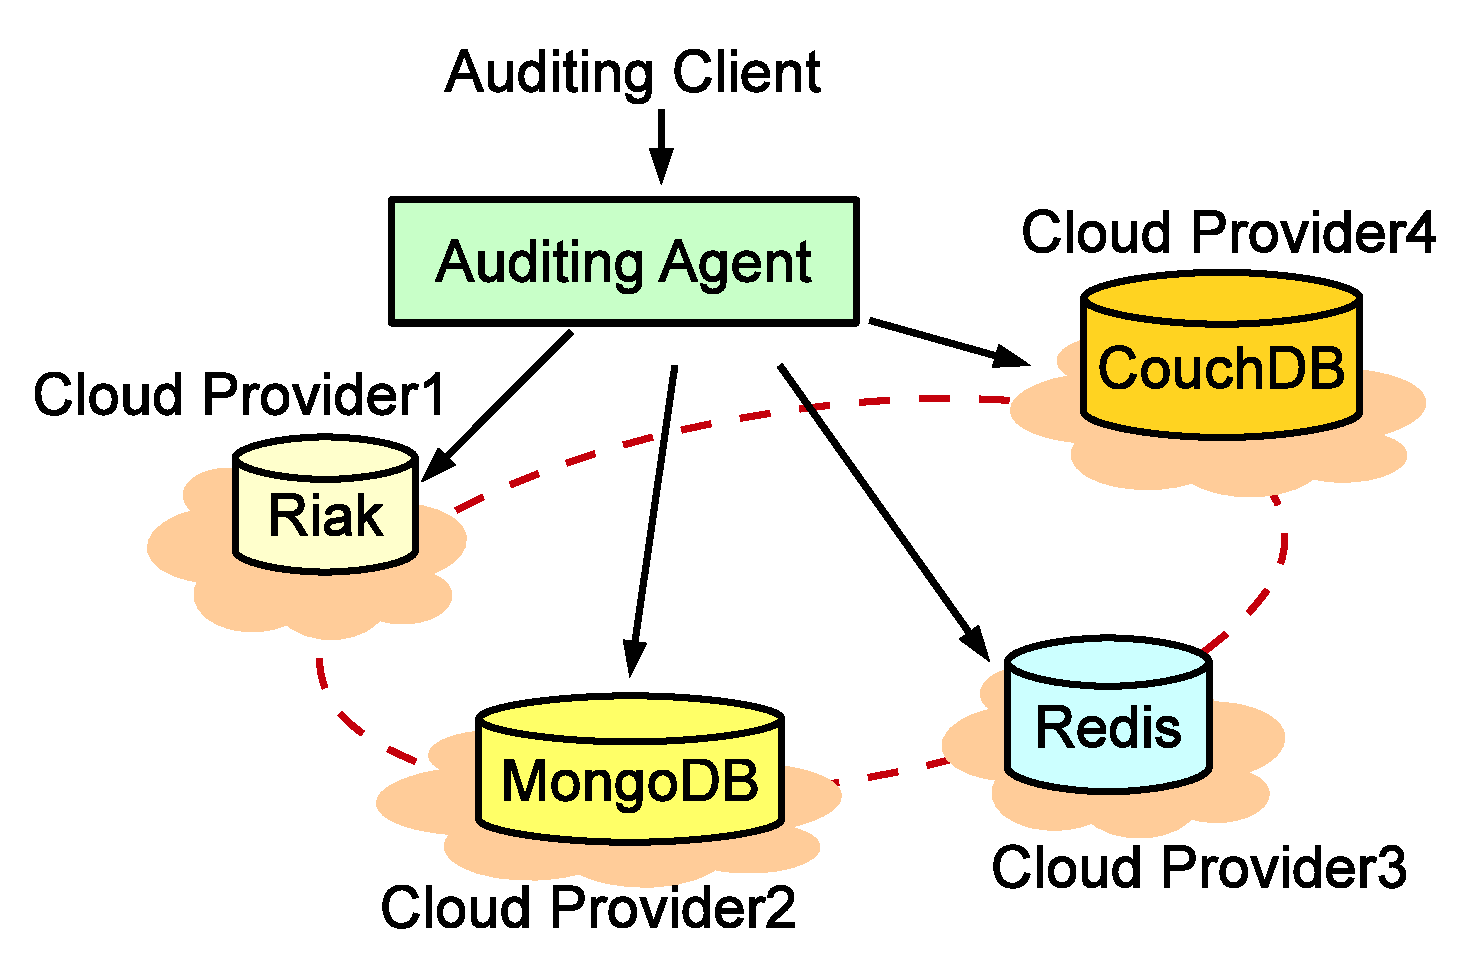
\includegraphics[width=0.94\textwidth]{figs/db.eps}
\caption{Case study for common software dependency.}
\label{fig-case3}
\end{figure}

The last case study targets a scenario where
\app offers private independence
auditing across multiple cloud providers.
In particular, a service provider,
Alice, wants a reliable storage solution
leveraging multiple cloud providers,
\eg, iCloud uses Amazon EC2 and Microsoft Azure for its reliable storage.
Suppose Alice has found four alternative cloud providers: Cloud~1-4,
each of which offers a key-value store.
Alice then consults \app for a redundancy deployment
%with the lowest number of common software dependencies
to avoid correlated failures caused by
any shared software dependency~\cite{greer14heartbleed}.

Here, we chose four popular key-value storage systems, \ie,
Riak, MongoDB, Redis, and CouchDB.
As shown in Figure~\ref{fig-case3},
we assigned each one to a cloud provider as follows,
Cloud1: Riak,
Cloud2: MongoDB,
Cloud3: Redis,
and Cloud4: CouchDB.
%Our experiment used four HP C7000 blades to run the storage systems,
%labeling them as ``Cloud1 Proxy'', ``Cloud2
%Proxy'', ``Cloud3 Proxy'' and ``Cloud4 Proxy'' respectively,
Suppose each cloud provider has used
our prototype to automatically collect the software dependencies
of the packages and libraries in its storage system.
Our \pia protocol privately computes the Jaccard similarity
for each potential redundancy deployment.
Table~\ref{tab-db} shows
the ranking lists of various two- and three-way
redundancy deployments.
We obtain Jaccard similarity without
using MinHash option for accurate independence scores.


